\section{Semaine 11 : 17/04/2023 - 21/04/2023}
\graphicspath{{semaines/semaine_11/images/}}

\begin{abstract}
	Après discussion avec Emmanuel vendredi 14/04, les points suivants vont être traités cette semaine :
	\begin{enumerate}[label=\textbullet]
		\item On cherchera dans un premier temps à comprendre pourquoi FEM n'a pas l'air de fonctionner aussi bien que PhiFEM en prenant $f=f_p$ et en faisant varier $\epsilon$.
		\item On va ensuite tester le rehaussement avec FEM et PhiFEM avec la solution exacte (sans perturbation, $\epsilon=0$).
		\item On ecrira ensuite les formulations pour le rehaussement avec PhiFEM "au propre".
		\item On testera ensuite d'appliquer les conditions limites pour PhiFEM différemment : on les impose de manière forte sur notre bord approché $\Gamma_h$.
	\end{enumerate}
	(Cette semaine, Michel est en vacance.)
\end{abstract}

\subsection{Correction et Rehaussement avec FEM}

Les résultats obtenus la semaine dernière pour FEM (dans la partie 10.2) semblait considérablement moins bon que PhiFEM. C'est pourquoi cette partie avait pour but de comprendre d'où provenait les problèmes dans les résultats. On s'est rendu compte qu'il fallait penser à bien distinguer les cas pour imposer les conditions aux bords sur $C$. 

\subsubsection*{Distinction des cas}

On considère ici le problème de Poisson avec condition de Dirichlet homogène et non homogène. 

On considère toujours qu'après une utilisation du FNO, on obtient une solution du type
$$u_p = u_{ex}+\epsilon P(x,y)$$

avec $u_{ex}$ la solution analytique définie par
$$u_{ex}(x,y) = S\times\sin(2\pi fx + \varphi)\times\sin(2\pi fy + \varphi)$$ 

et $P$ la perturbation définie par
$$P(x,y)=S_p\times\sin(2\pi f_px + \varphi_p)\times\sin(2\pi f_py + \varphi_p)$$

avec $\varphi_p=0$ pour que $P=0$ sur $\Gamma$ (et donc $u_p=u_{ex}$ sur $\Gamma$). 

On cherche alors à corriger cette solution avec et sans rehaussement.

On notera dans la suite $\tilde{u}$ la solution corrigée :
$$\tilde{u}=\tilde{\phi}C$$

\begin{enumerate}[label=\textbullet]
	\item \textbf{Problème homogène :}
	$$\left\{\begin{aligned}
		&-\Delta u=f \quad &&\Omega \\
		&u=0 \quad &&\Gamma
	\end{aligned}\right.$$

	\begin{itemize}
		\item \textbf{Correction :} ($m=0$)
		
		On pose
		$$\tilde{\phi}=u_p$$
		
		Et donc $\tilde{\phi}=0$ sur $\gamma$.
		
		On veut 
		$$\left\{\begin{aligned}
			&-\Delta(\tilde{\phi}C)=f \quad &&\Omega \\
			&\tilde{u}=0 \quad &&\Gamma
		\end{aligned}\right.$$
	
		Ce qui signifie que $\tilde{\phi}C=0$ sur $\Gamma$ et donc on ne sait pas la valeur de $C$ sur $\Gamma$ :
		$$C=\;? \quad\Gamma$$
		
		\begin{Rem}
			Si $f=f_p$, on a $C=\frac{u_{ex}}{(1+\epsilon)u_{ex}}=\frac{1}{1+\epsilon}$ sur $\Omega$ et donc on peut prendre $C=\frac{1}{1=\epsilon}$ sur $\Gamma$.
		\end{Rem}
	
		Une solution pour éviter ce problème est de rehausser la solution !
		
		\newpage
		\item \textbf{Rehaussement :}
		
		On pose
		$$\tilde{\phi}=u_p+m$$
		
		On veut 
		$$\left\{\begin{aligned}
			&-\Delta(\tilde{\phi}C)=f \quad &&\Omega \\
			&\tilde{u}=m \quad &&\Gamma
		\end{aligned}\right.$$
	
		Ainsi peu importe $f$ et $f_p$, on a 
		$$\left\{\begin{aligned}
			&C=\frac{u_{ex}+m}{\tilde{\phi}} \quad &&\Omega \\
			&C=1 \quad &&\Gamma
		\end{aligned}\right.$$
	
	\end{itemize}
	
	\item \textbf{Problème non homogène :}
	$$\left\{\begin{aligned}
		&-\Delta u=f \quad &&\Omega \\
		&u=g \quad &&\Gamma
	\end{aligned}\right.$$

	\begin{Rem}
		Dans le cas non homogène, on ne peut pas avoir $P=u_{ex}$ car $P=0$ sur $\Gamma$.
	\end{Rem}
	

	\begin{itemize}
		\item \textbf{Correction :} ($m=0$)
		
		On pose
		$$\tilde{\phi}=u_p$$
		
		Et donc $\tilde{\phi}=0$ sur $\gamma$.
		
		On veut 
		$$\left\{\begin{aligned}
			&-\Delta(\tilde{\phi}C)=f \quad &&\Omega \\
			&\tilde{u}=g \quad &&\Gamma
		\end{aligned}\right.$$
	
		Ainsi peu importe $f$ et $f_p$, on a 
		$$\left\{\begin{aligned}
			&C=\frac{u_{ex}}{u_{ex}+\epsilon P} \quad &&\Omega \\
			&C=1 \quad &&\Gamma
		\end{aligned}\right.$$
		
		\item \textbf{Rehaussement :}
		
		On pose
		$$\tilde{\phi}=u_p+m$$
		
		On veut 
		$$\left\{\begin{aligned}
			&-\Delta(\tilde{\phi}C)=f \quad &&\Omega \\
			&\tilde{u}=g+m \quad &&\Gamma
		\end{aligned}\right.$$
		
		Ainsi peu importe $f$ et $f_p$, on a 
		$$\left\{\begin{aligned}
			&C=\frac{u_{ex}+m}{\tilde{\phi}} \quad &&\Omega \\
			&C=1 \quad &&\Gamma
		\end{aligned}\right.$$
	\end{itemize}

\end{enumerate}

\subsubsection*{Problème initial}

On se place dans le cas où on avait obtenu les problèmes la semaine précédente, c'est-à-dire dans le cas du problème de Poisson avec condition de Dirichlet homogène avec $f=f_p$. 

Au vue de la sous-section précédente, il semblerait que le problème obtenue vienne de la condition de bord imposée à FEM pour $C$ (qui était $C=1$ sur $\Gamma$). En effet, voici les résultats obtenus avec cette condition :

\begin{minipage}{\linewidth}
	\centering
	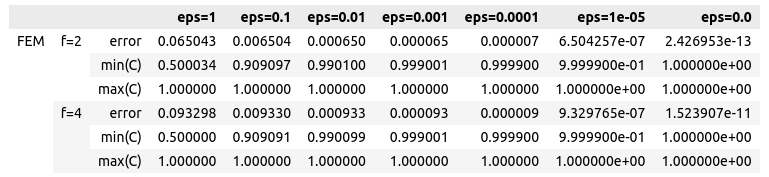
\includegraphics[width=0.8\linewidth]{test1_avant.png}
\end{minipage}

En modifiant cette condition par $C=\frac{1}{1+\epsilon}$, on a


\begin{minipage}{\linewidth}
	\centering
	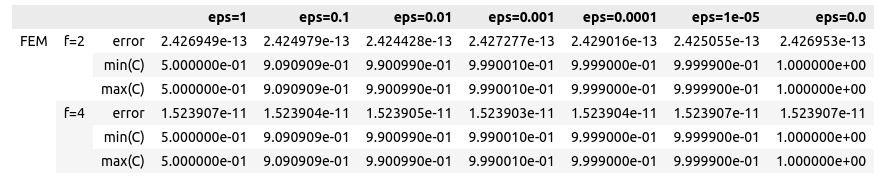
\includegraphics[width=0.8\linewidth]{test1_apres.png}
\end{minipage}

En prenant $f=2$ et $\epsilon=1$, on obtient les résultats suivants (à gauche le $C$ obtenu par FEM en imposant $C=1$ sur $\Gamma$, au milieu le $C$ obtenu par FEM en imposant $C=\frac{1}{1+\epsilon}$ sur $\Gamma$ et à droite notre solution analytique $u_{ex}$) :

\begin{minipage}{\linewidth}
	\centering
	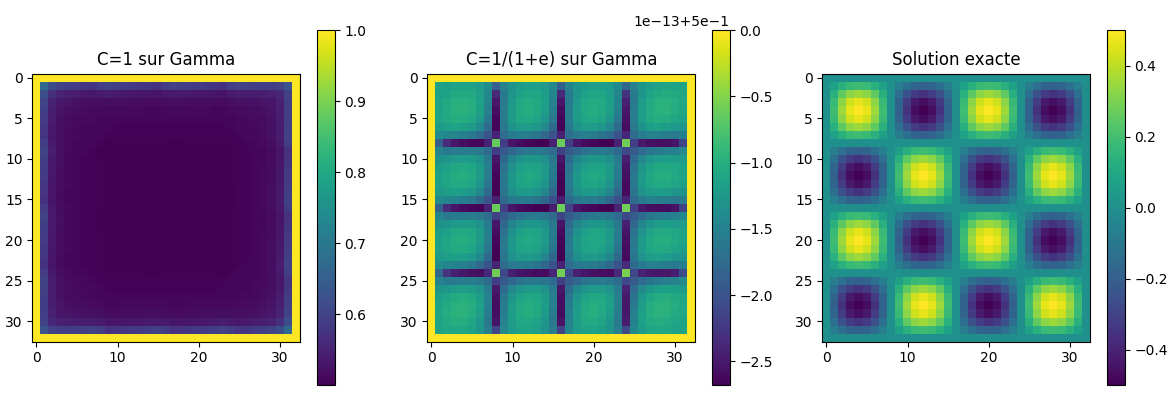
\includegraphics[width=0.8\linewidth]{test1_C.png}
\end{minipage}

\subsubsection*{Résultats supplémentaires}

En tant que vérification supplémentaire des résultats obtenus dans la distinction des cas, on va comparer le $C$ obtenu par FEM et le $C$ analytique dans les différents cas considérés où l'on rehausse la solution. On considerera dans la suite $S=0.5$ et $m=100$.

\begin{enumerate}[label=\textbullet]
	\item \textbf{Problème homogène :} $\varphi=0$
	
	Pour $f=f_p=2$, on obtient les résultats suivants (avec $\epsilon=1e-5$ et nb\_vert=64) :
	
	\begin{minipage}{\linewidth}
		\centering
		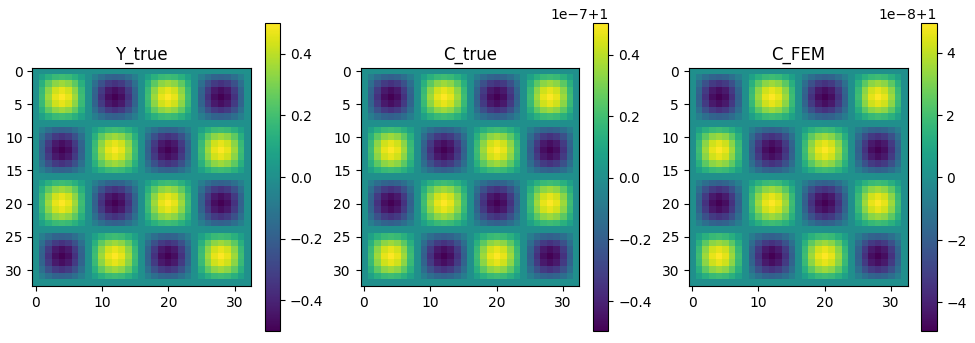
\includegraphics[width=0.7\linewidth]{test2_homo_egal.png}
	\end{minipage}

	En faisant varier $\epsilon$, on obtient les résultats numérique suivants :
	
	\begin{minipage}{\linewidth}
		\centering
		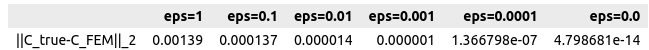
\includegraphics[width=0.7\linewidth]{test2_homo_egal_eps.png}
	\end{minipage}
	
	Pour $f=4$ et $f_p=2$, on obtient les résultats suivants (avec $\epsilon=1e-5$ et nb\_vert=64) :
	
	\begin{minipage}{\linewidth}
		\centering
		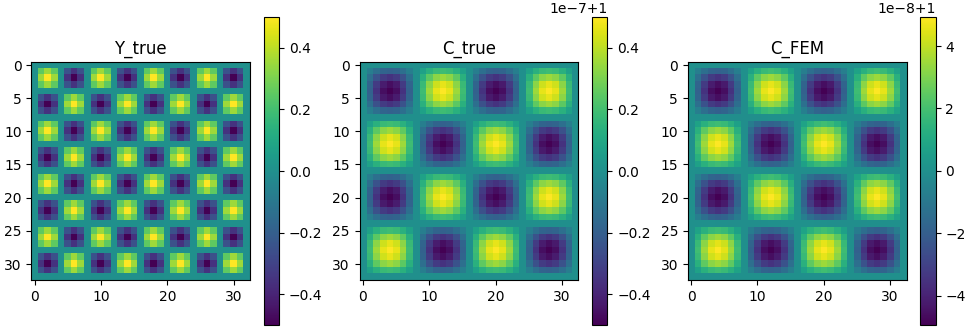
\includegraphics[width=0.7\linewidth]{test2_homo_diff.png}
	\end{minipage}
	
	En faisant varier $\epsilon$, on obtient les résultats numérique suivants :
	
	\begin{minipage}{\linewidth}
		\centering
		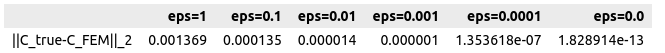
\includegraphics[width=0.7\linewidth]{test2_homo_diff_eps.png}
	\end{minipage}
	
	\newpage
	
	\item \textbf{Problème non homogène :} $\varphi=1$
	
	Pour $f=4$ et $f_p=2$, on obtient les résultats suivants (avec $\epsilon=1e-5$ et nb\_vert=64) :
	
	\begin{minipage}{\linewidth}
		\centering
		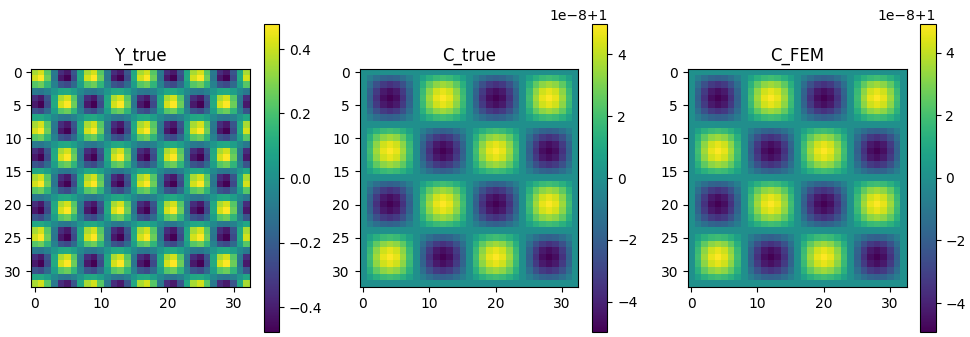
\includegraphics[width=0.7\linewidth]{test2_non_homo.png}
	\end{minipage}
	
	En faisant varier $\epsilon$, on obtient les résultats numérique suivants :
	
	\begin{minipage}{\linewidth}
		\centering
		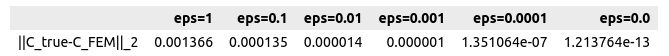
\includegraphics[width=0.7\linewidth]{test2_non_homo_eps.png}
	\end{minipage}
	
\end{enumerate}

\subsection{Rehaussement PhiFEM}

On considère le problème de Poisson avec condition de Dirichlet homogène :
$$\left\{\begin{aligned}
	&-\Delta u=f \quad &&\Omega \\
	&u=0 \quad &&\Gamma
\end{aligned}\right.$$

On se place encore sur le carré $[0,1]^2$. Pour construire nos ensembles, on utilisera
$$\phi_c (x)=||x-0.5||_\infty-0.5$$

On considérera le domaine environnant $\mathcal{O}=[-0.5,1.5]^2$.

Pour PhiFEM, on prendra la levelset
$$\phi (x,y)=x(1-x)y(1-y)$$

On considère encore la solution analytique suivante :
$$u_{ex}(x,y) = S\times\sin(2\pi fx + \varphi)\times\sin(2\pi fy + \varphi)$$ 

et pour $p=0$, $g(x,y)=0$.

De la même manière que pour FEM, on va considérer la solution rehaussée par $m$ :
$$\tilde{\phi}=u_p+m$$
avec
$$u_p=u_{ex}+\epsilon P$$

\begin{Rem}
	Ici $\tilde{\phi}=m$ sur $\Gamma$ (et $u_p=0$ sur $\Gamma$).
\end{Rem}

On cherche alors à résoudre le problème
$$\left\{\begin{aligned}
	&-\Delta(\tilde{\phi}C)=f \quad &&\Omega \\
	&\tilde{u}=m \quad &&\Gamma
\end{aligned}\right.$$

On testera d'imposer les conditions aux bords de deux manières :
\begin{itemize}
	\item 1ère méthode : Comme $\tilde{\phi}=m$ sur $\Gamma$ (et pas 0), on ne fais rien !
	\item 2ème méthode : On cherche à imposer $C=1$ sur $\Gamma_h$ (2 cas à différencier : nb\_vert=64 et nb\_vert=101).
\end{itemize}

On testera dans un premier temps les 2 méthodes pour $\epsilon=0$ (c'est-à-dire sans perturbation) puis pour différents $\epsilon\ne 0$ (avec perturbation).

\subsubsection*{Sans perturbation ($\epsilon=0$)}

On testera pour différentes fréquences avec $f=f_p$. On prendra $\epsilon=0$ et on fera varier $m$.

\begin{enumerate}[label=\textbullet]
	\item \textbf{Ancienne version :} (avec ajout des termes en $g$)
	
	Voici les résultats numériques obtenus (à gauche les erreurs et à droite les facteurs) :
	
	\begin{minipage}{0.52\linewidth}
		\centering
		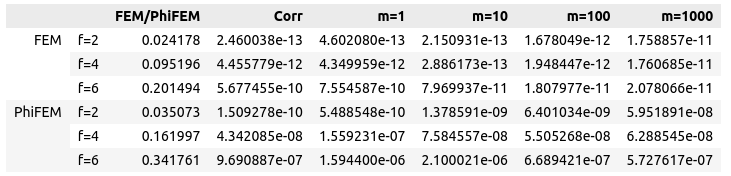
\includegraphics[width=\linewidth]{test3_sans_0_erreur.png}
	\end{minipage}
	\begin{minipage}{0.44\linewidth}
		\centering
		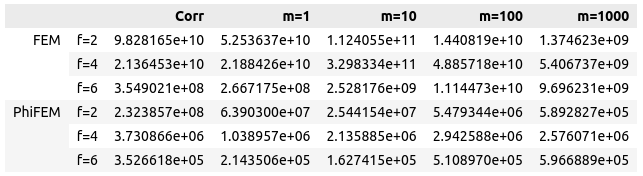
\includegraphics[width=\linewidth]{test3_sans_0_facteur.png}
	\end{minipage}
	
	En traçant les erreurs FEM et PhiFEM pour différentes fréquences $f$ en fonction du rehaussement $m$, on obtient :
	
	\begin{minipage}{\linewidth}
		\centering
		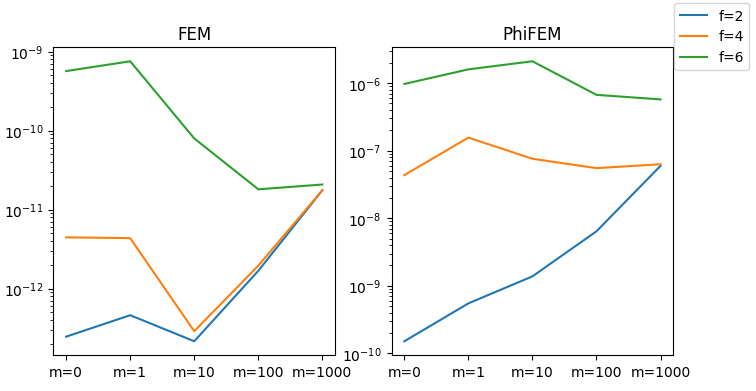
\includegraphics[width=0.5\linewidth]{test3_sans_0_courbes.png}
	\end{minipage}

	\item \textbf{1ère méthode :} (on fait rien !)
	
	Voici les résultats numériques obtenus (à gauche les erreurs et à droite les facteurs) :
	
	\begin{minipage}{0.48\linewidth}
		\centering
		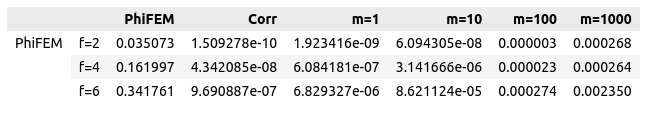
\includegraphics[width=\linewidth]{test3_sans_1_erreur.png}
	\end{minipage}
	\begin{minipage}{0.48\linewidth}
		\centering
		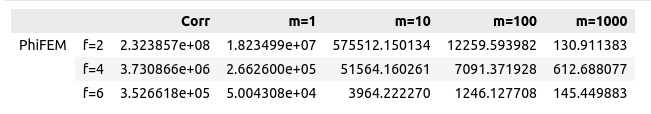
\includegraphics[width=\linewidth]{test3_sans_1_facteur.png}
	\end{minipage}
	
	En traçant les erreurs PhiFEM pour différentes fréquences $f$ en fonction du rehaussement $m$, on obtient :
	
	\begin{minipage}{\linewidth}
		\centering
		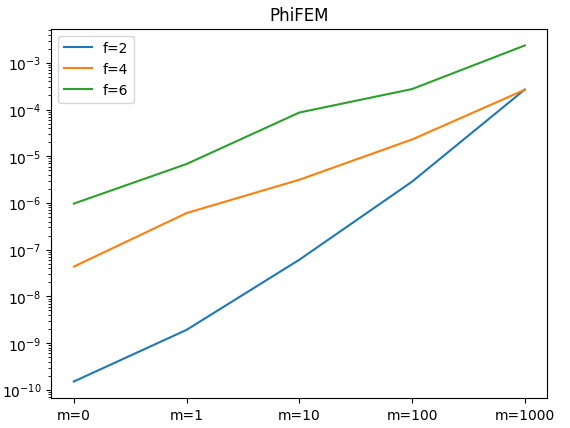
\includegraphics[width=0.3\linewidth]{test3_sans_1_courbes.png}
	\end{minipage}
	
	\item \textbf{2ème méthode : nb\_vert=101}
	
	Voici les résultats numériques obtenus (à gauche les erreurs et à droite les facteurs) :
	
	\begin{minipage}{0.48\linewidth}
		\centering
		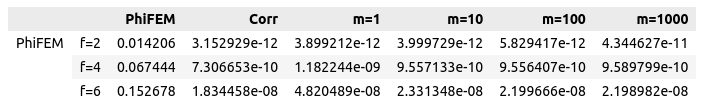
\includegraphics[width=\linewidth]{test3_sans_2a_erreur.png}
	\end{minipage}
	\begin{minipage}{0.48\linewidth}
		\centering
		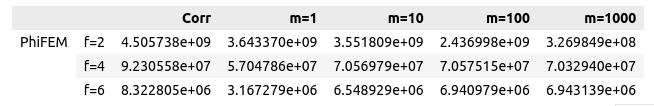
\includegraphics[width=\linewidth]{test3_sans_2a_facteur.png}
	\end{minipage}
	
	En traçant les erreurs PhiFEM pour différentes fréquences $f$ en fonction du rehaussement $m$, on obtient :
	
	\begin{minipage}{\linewidth}
		\centering
		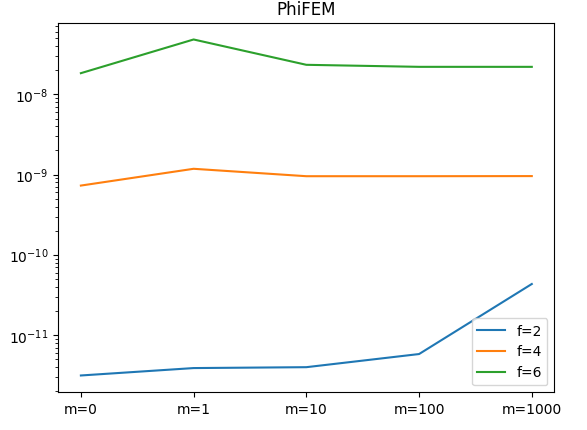
\includegraphics[width=0.3\linewidth]{test3_sans_2a_courbes.png}
	\end{minipage}
	
	\newpage
	\item \textbf{2ème méthode : nb\_vert=64}
	
	Voici les résultats numériques obtenus (à gauche les erreurs et à droite les facteurs) :
	
	\begin{minipage}{0.48\linewidth}
		\centering
		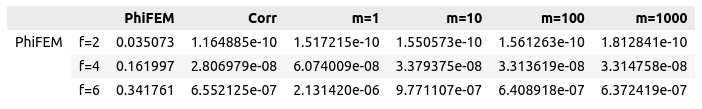
\includegraphics[width=\linewidth]{test3_sans_2b_erreur.png}
	\end{minipage}
	\begin{minipage}{0.48\linewidth}
		\centering
		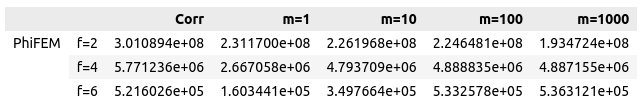
\includegraphics[width=\linewidth]{test3_sans_2b_facteur.png}
	\end{minipage}
	
	En traçant les erreurs PhiFEM pour différentes fréquences $f$ en fonction du rehaussement $m$, on obtient :
	
	\begin{minipage}{\linewidth}
		\centering
		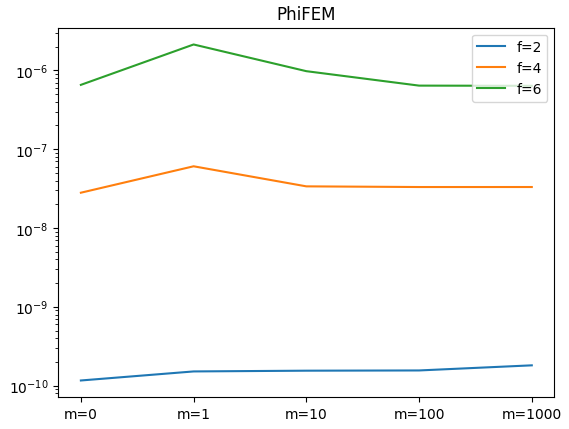
\includegraphics[width=0.3\linewidth]{test3_sans_2b_courbes.png}
	\end{minipage}
	
\end{enumerate}


\subsubsection*{Avec perturbation ($\epsilon\ne 0$)}


On testera pour différentes fréquences avec $f\ne f_p$. On prendra $\epsilon=0.01$ et $\epsilon=0.001$ et on fera varier $m$.

\begin{enumerate}[label=\textbullet]
	\item \textbf{1ère méthode :} (on fait rien !)
	
	Voici les résultats numériques obtenus :
	
	\begin{minipage}{\linewidth}
		\centering
		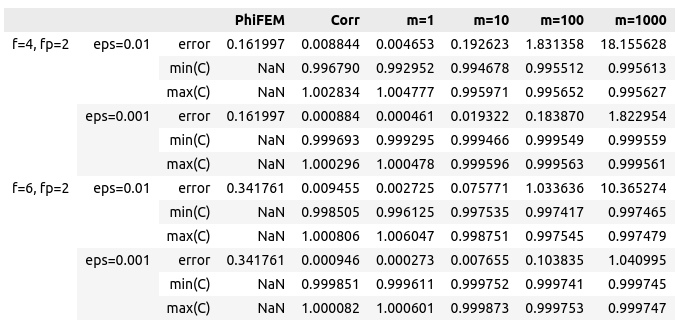
\includegraphics[width=0.6\linewidth]{test3_avec_1_erreur.png}
	\end{minipage}
	
	En traçant les erreurs PhiFEM pour différentes fréquences $f$ en fonction du rehaussement $m$, on obtient :
	
	\begin{minipage}{\linewidth}
		\centering
		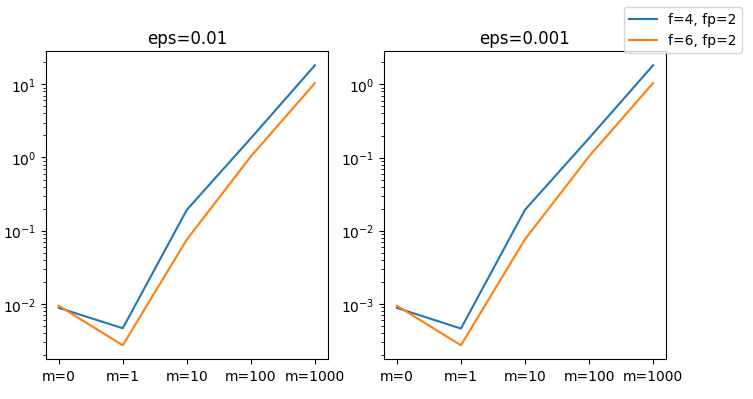
\includegraphics[width=0.6\linewidth]{test3_avec_1_courbes.png}
	\end{minipage}
	
	\newpage
	
	\item \textbf{2ème méthode : nb\_vert=101}
	
	Voici les résultats numériques obtenus :
	
	\begin{minipage}{\linewidth}
		\centering
		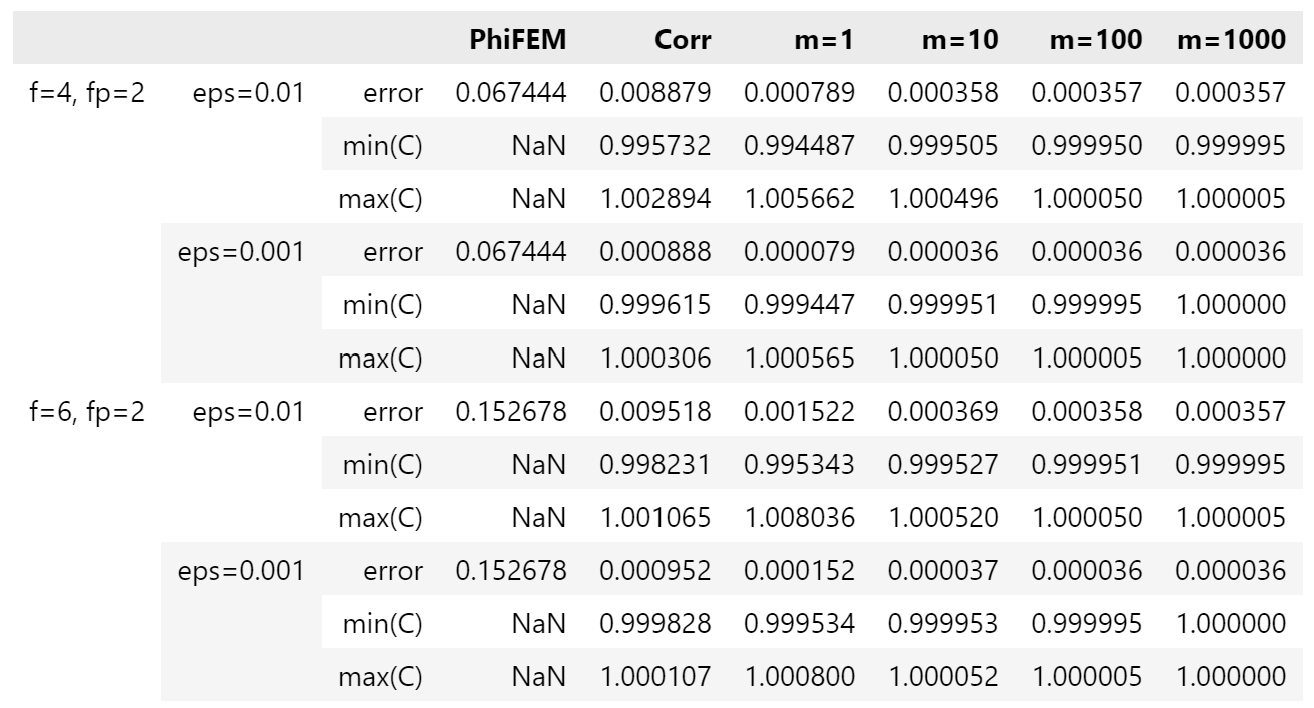
\includegraphics[width=0.6\linewidth]{test3_avec_2a_erreur.png}
	\end{minipage}
	
	En traçant les erreurs PhiFEM pour différentes fréquences $f$ en fonction du rehaussement $m$, on obtient :
	
	\begin{minipage}{\linewidth}
		\centering
		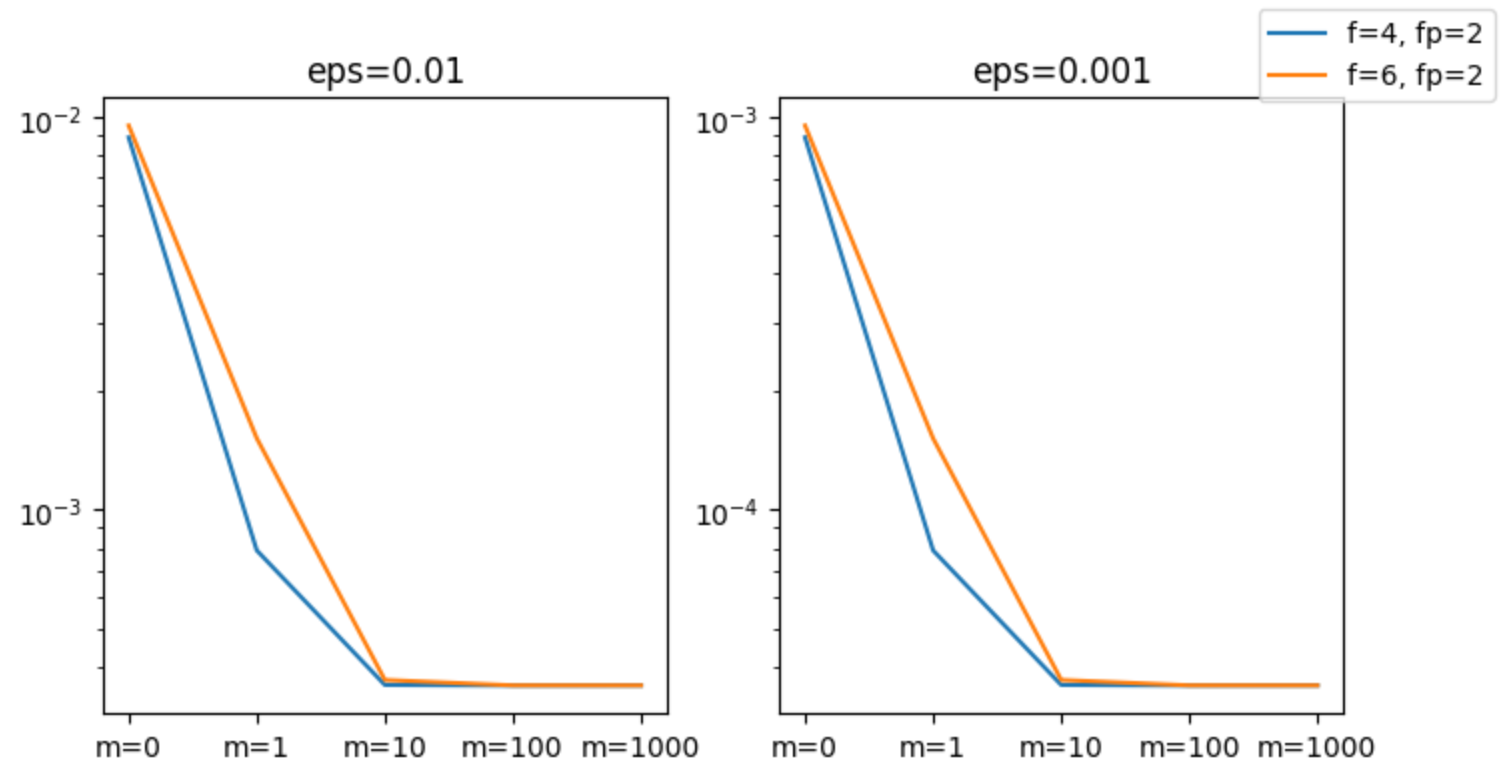
\includegraphics[width=0.6\linewidth]{test3_avec_2a_courbes.png}
	\end{minipage}
	
	\item \textbf{2ème méthode : nb\_vert=64}
	
	Voici les résultats numériques obtenus :
	
	\begin{minipage}{\linewidth}
		\centering
		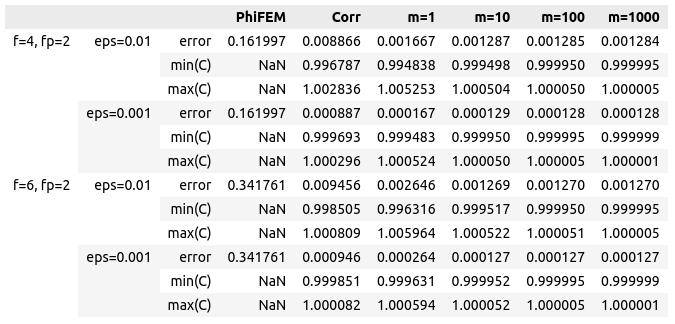
\includegraphics[width=0.6\linewidth]{test3_avec_2b_erreur.png}
	\end{minipage}
	
	En traçant les erreurs PhiFEM pour différentes fréquences $f$ en fonction du rehaussement $m$, on obtient :
	
	\begin{minipage}{\linewidth}
		\centering
		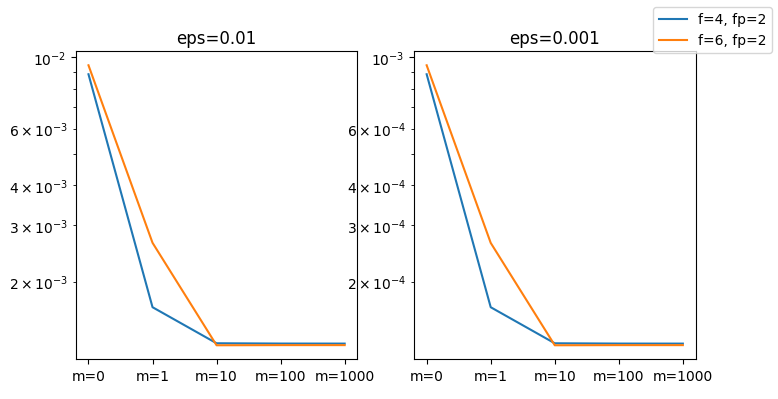
\includegraphics[width=0.6\linewidth]{test3_avec_2b_courbes.png}
	\end{minipage}
	
\end{enumerate}